\documentclass[10pt,hyperref={CJKbookmarks=true},xcolor=dvipsnames,aspectratio=169]{beamer}
\usetheme[navigation]{UMONS}
\usepackage[utf8]{inputenc}
\usepackage{verbatim}
\usepackage{ctex}

\title[国际经济学]{国际经济学}
\subtitle{国际货币体系:历史视角}
\author{鲁晓东}
\institute[]{%
	岭南学院\hspace{2em}中山大学
	\\[4ex]
	
\includegraphics[height=8ex]{fig/lingnanlogo}\hspace{2em}%
	
\includegraphics[height=8.5ex]{fig/sysu}
}
%------------section前展示一页----------
\AtBeginSection[] {     
	\begin{frame}        
	\tableofcontents[currentsection,hideallsubsections]    
\end{frame} 
}

%-------------subsection也展示一下----------
\AtBeginSubsection[]{

\frame<beamer>{ 
	
	\frametitle{Outline}   
	
	\tableofcontents[currentsection,currentsubsection] 
	
}

}
%---------------------------

%-----------一段一闪现-------
%\beamerdefaultoverlayspecification{<+->}
%这个功能基本不用

\begin{document}
\maketitle


\begin{frame}
\frametitle{提纲}
\tableofcontents
\end{frame}				%生成提纲页

%-----------正文开始----------------------



\section{Motivation}
\begin{frame}{Quotation from Keynes}
\begin{itemize}
	\item 事实上,\textcolor{red}{金本位已经是个野蛮的遗迹}。现在,从英格兰银行行长到我们普通人都主要对保持商业、价格和就业的稳定性感兴趣,并且当我们面临选择时,我们不可能故意为了陈腐教条做出这些牺牲$\cdots$古典本位思想的拥护者没有意识到他现在已经远离时代的精神和要求。\\
	——梅纳德$\cdot$凯恩斯,1923
\end{itemize}
\centering
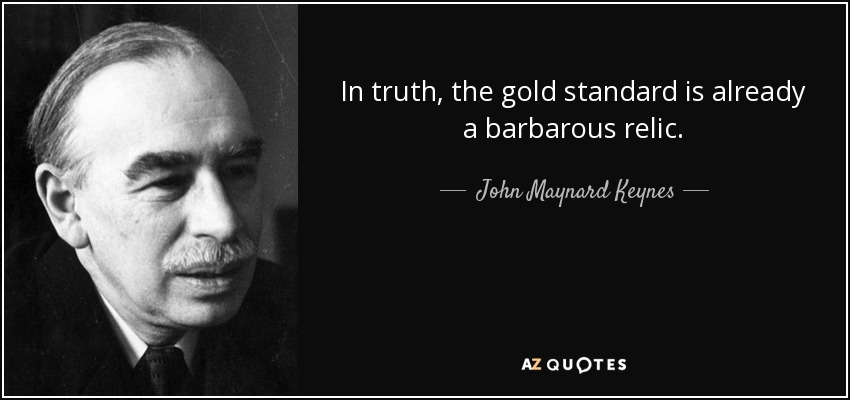
\includegraphics[scale=0.3]{fig/systems/keynes}
\end{frame}

	
\begin{frame}{Quatation from Friedman}

\begin{columns}[onlytextwidth]
	\begin{column}{0.4\textwidth}
		\begin{itemize}
			\item 有责任心的人们最终确信,钉住汇率对具有独立的政治系统和独立的国家政策的大国而言不是一种的满意的金融安排,而在这之前,还会有多少惨痛的失败教训?\\
			---米尔顿 弗雷德曼,1992 
		\end{itemize}
	\end{column}
	\begin{column}{0.6\textwidth}
		\centering
		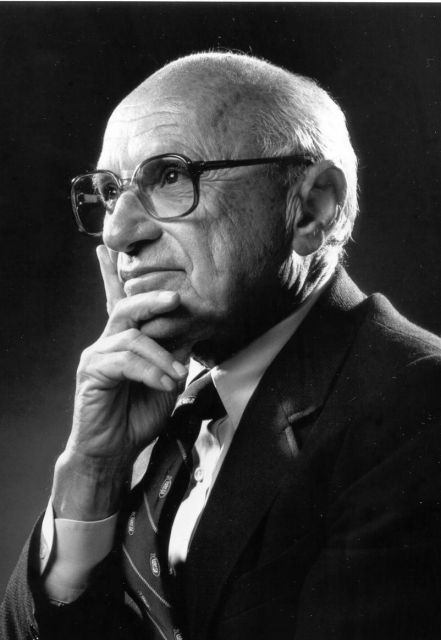
\includegraphics[scale=0.3]{fig/systems/friedman}
	\end{column}
\end{columns}

\end{frame}

\begin{frame}{Quatation from Ronald I. Mckinnon}

\begin{columns}[onlytextwidth]
	\begin{column}{0.6\textwidth}
		\begin{itemize}
	\item 尤其是金本位——甚至是一般意义上的钉住汇率制——名声不佳。虽然在20世纪20-30年代金本位逐渐失去了他的名声,但人们不应因此而忘记它在19世纪的优点。$\cdots$为这个野蛮的遗迹所束缚的世界已经不复存在,还能找回那些失落已久的优点吗?$\cdots$在一个一体化的世界经济里,汇率制度的选择——从而共同的价格水平的选择——不只是单单一个国家的事情。其溢出效应如此之高,以致它应该是一件集体选择的事情。\\
	——罗纳德$\cdot$麦金农,美国斯坦福大学教授,当代金融发展理论奠基人
		\end{itemize}
	\end{column}
	\begin{column}{0.4\textwidth}
		\centering
		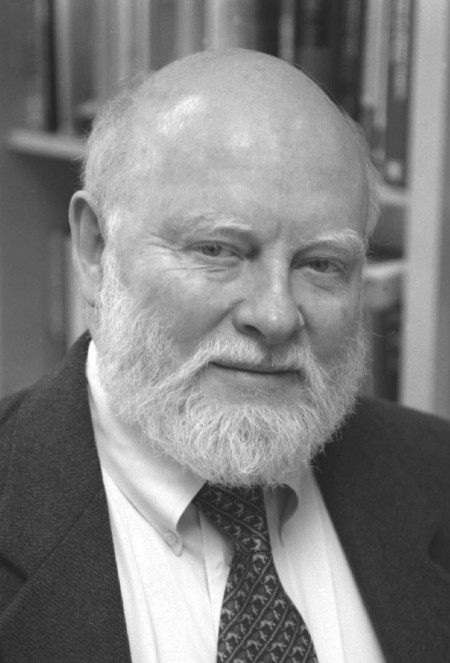
\includegraphics[scale=0.3]{fig/systems/mckinnon}
	\end{column}
\end{columns}
\end{frame}

\begin{frame}{A Spectrum of Exchange Rate Regimes }
\centering
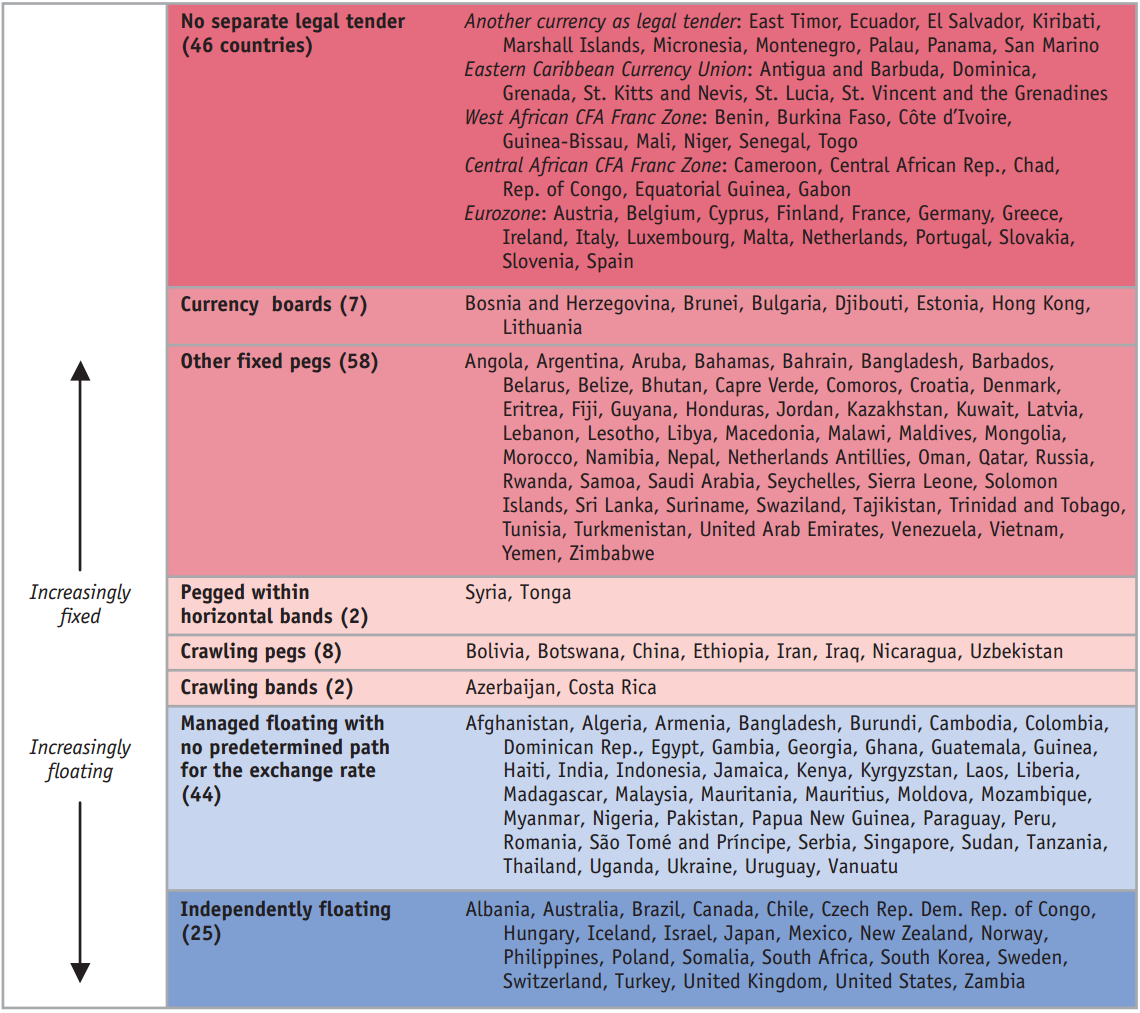
\includegraphics[scale=0.28]{fig/systems/spectrum}
\begin{itemize}
	\item The chart shows
	a recent classification of exchange rate regimes around the
	world.
	\item There is no 'right' regime in exchange rate, all things are depend.
\end{itemize}
\end{frame}

\section{宏观经济政策目标:内外平衡}

\begin{frame}{Macroeconomic Goals}
	\begin{itemize}
		\item “Internal balance” describes the macroeconomic goals of
		producing at \structure{potential output} (at “full employment”) and of \structure{price stability} (low inflation).
		\begin{itemize}
			\item An unsustainable use of resources (overemployment) tends to		increase prices; an ineffective use of resources
			(underemployment) tends to decrease prices.
		\end{itemize}
	\item Volatile aggregate demand and output tend to create volatile
	prices.
			\begin{itemize}
		\item Price level movements reduce the economy’s efficiency by
		making the real value of the monetary unit less certain and thus
		a less useful guide for economic decisions.
	\end{itemize}
	\item “External balance” achieved when a current account is
				\begin{itemize}
		\item neither so deeply in deficit that the country may be unable to
		repay its foreign debts,
		\item nor so strongly in surplus that foreigners are put in that position.
		\begin{itemize}
			\item For example, pressure on Japan in the 1980s and China in the 2000s.
		\end{itemize}
	\end{itemize}
	
	\end{itemize}
\end{frame}

\begin{frame}{The Open-Economy Trilemma}
\begin{columns}[onlytextwidth]
	\begin{column}{0.6\textwidth}
		\begin{itemize}
			\item Exchange rate stability.
			\item Monetary policy oriented toward domestic goals.
			\item Freedom of international capital movements.
		\end{itemize}
	\end{column}
	\begin{column}{0.4\textwidth}
		\centering
		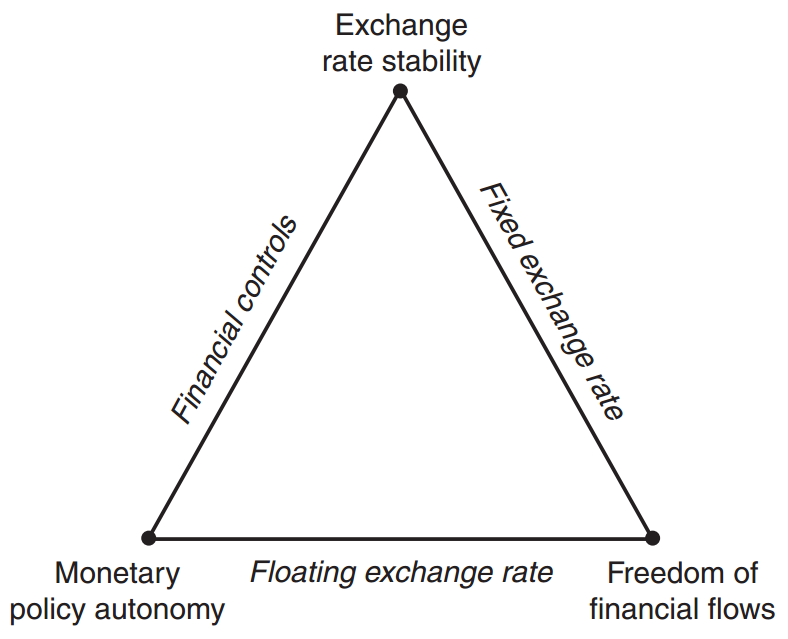
\includegraphics[scale=0.3]{fig/systems/trilemma}
	\end{column}
\end{columns}
\end{frame}


\section{金本位制:1870-1914}
\begin{frame}{Origins of the Gold Standard}
	\begin{itemize}
		\item The gold standard from 1870 to 1914 and after
		1918 had mechanisms that prevented flows of gold
		reserves (the balance of payments) from becoming
		too positive or too negative.
		\begin{itemize}
			\item  Prices tended to adjust according the amount of gold
			circulating in an economy, which had effects on the flows
			of goods and services: the current account.
			\item  Central banks influenced financial asset flows, so that the
			nonreserve part of the financial account matched the
			current account in order to reduce gold outflows or
			inflows.
		\end{itemize}
	\end{itemize}
\end{frame}

\begin{frame}{Price-specie-flow mechanism}
\begin{itemize}
	\item \structure{Price-specie-flow mechanism} is the adjustment
	of prices as gold (“specie”) flows into or out of a
	country, causing an adjustment in the flow of
	goods.
	\begin{itemize}
		\item  Prices tended to adjust according the amount of gold
		circulating in an economy, which had effects on the flows
		of goods and services: the current account.
		\item  Central banks influenced financial asset flows, so that the
		nonreserve part of the financial account matched the
		current account in order to reduce gold outflows or
		inflows.
	\end{itemize}
\end{itemize}
\end{frame}

\begin{frame}{Why we think Gold Standard is a fixed exchagne rate regime}
	\begin{itemize}
		\item 铸币平价:1英镑=4.8665美元。输送黄金的额外费用约0.0292美元/英镑
		\item 本币贬值足够低,使得用本币购买外币成本过高,而将本币变成黄金输出到外国再改铸成外币的成本更低,则出现本国黄金输出点(对外国为输入点)。
		\item 反之,当本币升值足够高,使得用外币购买本币过高,而将外币变成黄金输入到本国再改铸成本币的成本更低,则出现本国黄金输入点(对外国为输出点)。
	\end{itemize}
		\centering
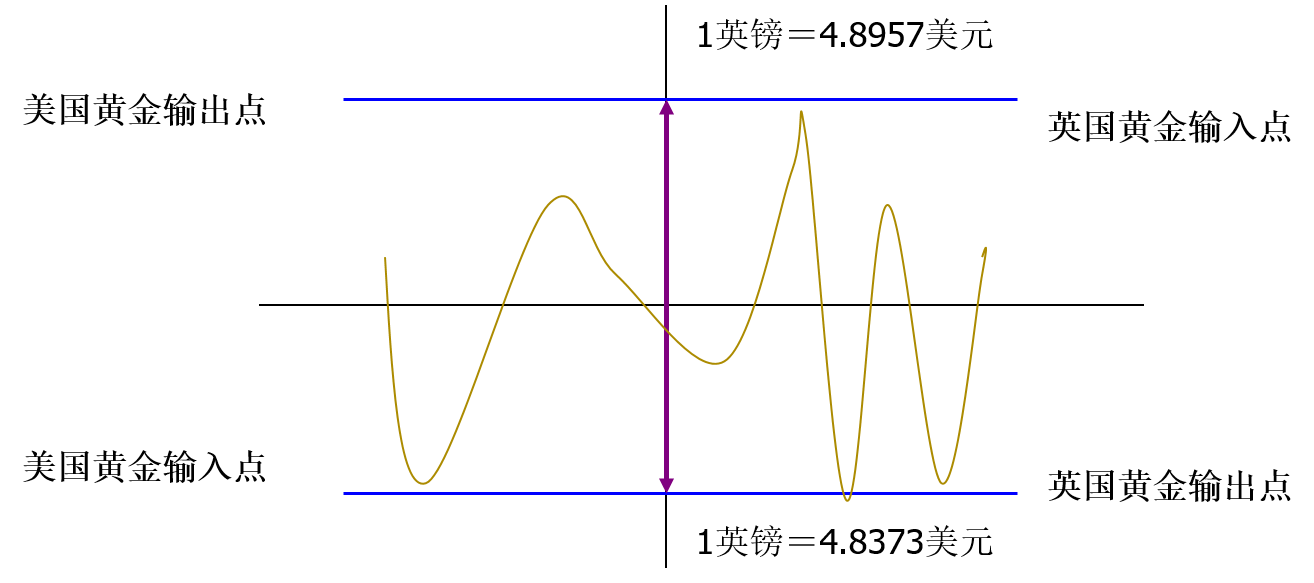
\includegraphics[scale=0.4]{fig/systems/specie}
\end{frame}

\begin{frame}{The “Rules of the Game” under the gold standard}
\begin{itemize}
	\item In theory, the price-specie-flow mechanism could operate automatically. But the
	reactions of central banks to gold flows across their borders furnished another
	potential mechanism to help restore balance of payments equilibrium. 
	\item The \structure{“Rules of the Game”} under the gold standard
	refer to another adjustment process that was
	theoretically carried out by central banks
	\begin{itemize}
		\item The selling of domestic assets to acquire money when gold
		exited the country as payments for imports.减少黄金流出
		\item The buying of domestic assets when gold enters the
		country as income from exports. 减少黄金流入
	\end{itemize}
\end{itemize}
\end{frame}
\begin{frame}{The gold standard’s record for internal balance was
	mixed}

\begin{columns}[onlytextwidth]
	\begin{column}{0.6\textwidth}
		\begin{itemize}
		
				\item The gold standard’s record for internal balance was
				mixed.
			\begin{itemize}
			\item The U.S. suffered from deflation, recessions, and financial
			instability during the 1870s, 1880s, and 1890s while
			trying to adhere to a gold standard.
			\item The U.S. unemployment rate was 6.8\% on average from
			1890 to 1913, but it was less than 5.7\% on average from
			1946 to 1992.
		\end{itemize}	
	\end{itemize}
	\end{column}
	\begin{column}{0.4\textwidth}
		\centering
		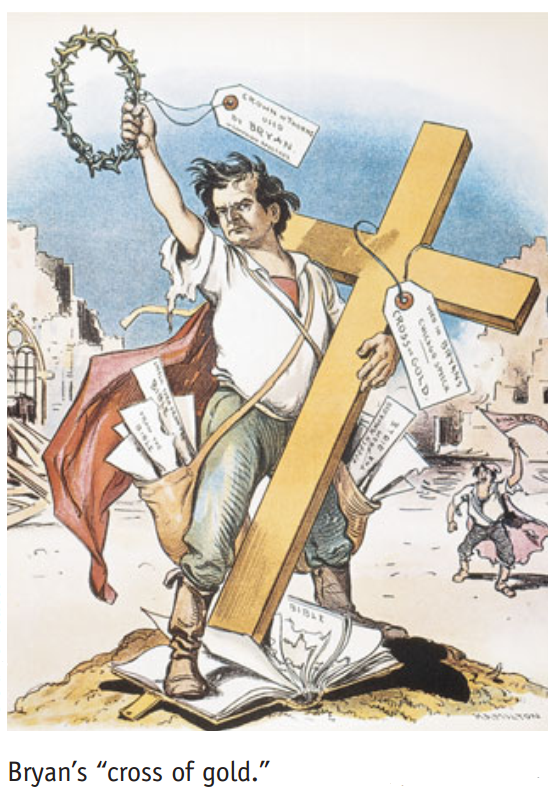
\includegraphics[scale=0.3]{fig/systems/bryan}
	\end{column}
\end{columns}

\end{frame}
\begin{frame}{Comments on Gold Standard}
		\begin{itemize}[<+->]
	\item 汇率稳定,促进全球贸易、世界经济发展
	\item 世界能否重回金本位时代?
	\item 黄金是否还是货币?
	\item 黄金能否重拾货币荣耀?
		\begin{itemize}
			\item 恢复金平价?有黄金虫(gold bug)倡导,但不可能
			\item 黄金产量有限
			\item 货币需求量太大
			\item 纸币时代、电子货币时代,早就不是用金子银子的时代了!
		\end{itemize}
\end{itemize}
\end{frame}

\section{两次世界大战期间:1918-1939}
\begin{frame}{The Fleeting Return to Gold}
		\begin{itemize}
	\item The gold standard was stopped in 1914 due to war,
	but after 1918 it was attempted again
		\begin{itemize}
		\item The U.S. reinstated the gold standard from 1919 to 1933
		at \$20.67 per ounce and from 1934 to 1944 at \$35.00 per
		ounce (a devaluation of the dollar).
		\item The U.K. reinstated the gold standard from 1925 to 1931.
	\end{itemize}
	\item But countries that adhered to the gold standard for
	the longest time, without devaluing their
	currencies, suffered most from reduced output and
	employment during the 1930s.
	

\end{itemize}
\end{frame}

\section{布雷顿森林体系:1944-1973}
\begin{frame}{44 countries meeting in Bretton Woods}
	\begin{itemize}
		\item In July 1944, 44 countries met in Bretton Woods,
		NH, to design the Bretton Woods system:
		\begin{itemize}
			\item a fixed exchange rate against the U.S. dollar and a fixed
			dollar price of gold (\$35 per ounce).
		\end{itemize}
	\item They also established other institutions:
	\begin{itemize}
		\item The International Monetary Fund
		\item The World Bank
		\item General Agreement on Trade and Tariffs (GATT), the
		predecessor to the World Trade Organization (WTO).
	\end{itemize}
	\end{itemize}
\end{frame}

\begin{frame}{The History of Bretton Woods}
	\centering
	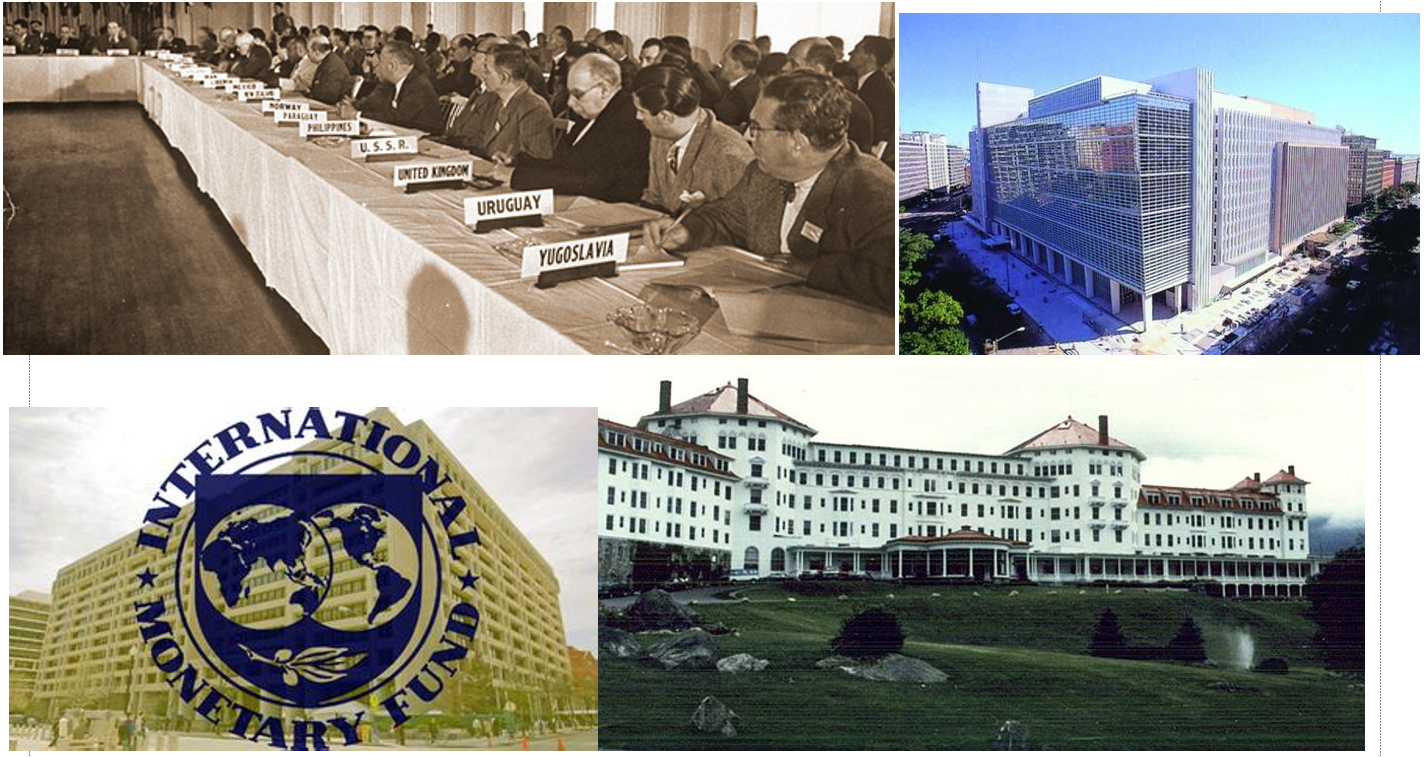
\includegraphics[scale=0.46]{fig/systems/bretton}
\end{frame}

\begin{frame}{The Current View of Bretton Woods}
\centering
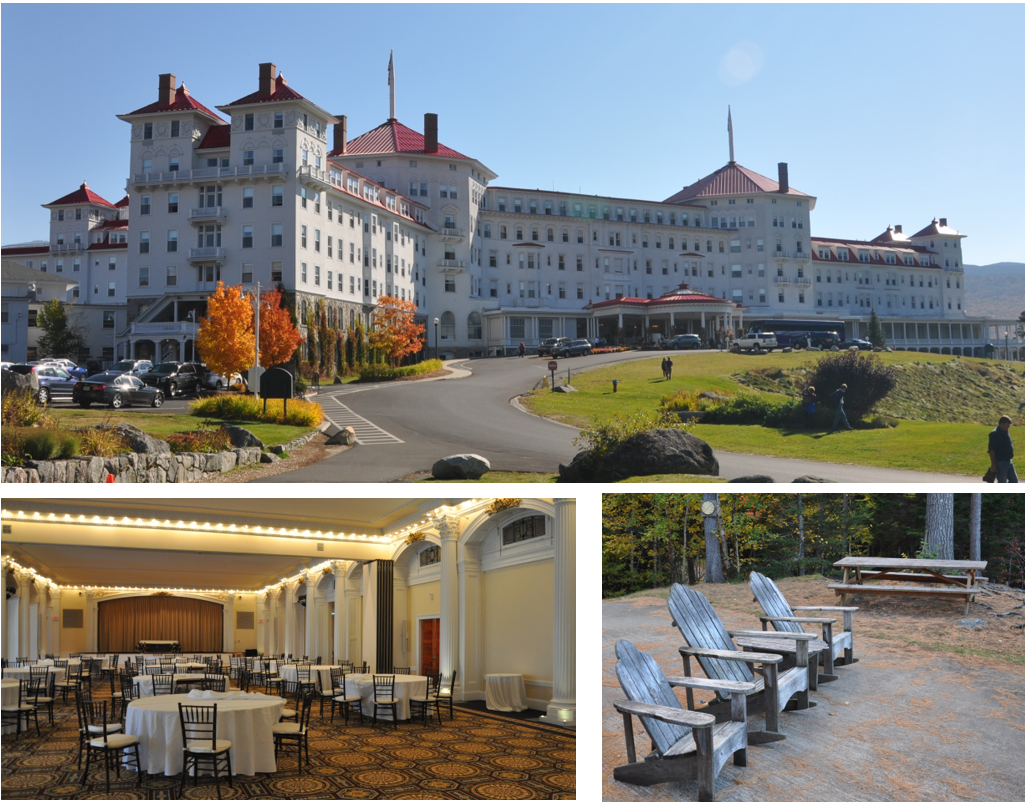
\includegraphics[scale=0.4]{fig/systems/bretton2}
\end{frame}

\begin{frame}{the brief history of bretton woods}
	\begin{itemize}
		\item 1974年3月正式生效
		\item 各国无力获取美元$\longrightarrow$马歇尔计划$\longrightarrow$OECD组织建立$\longrightarrow$50年代,美国的顺差转为逆差$\longrightarrow$黄金外流$\longrightarrow$ 1961年借款总协议(GAB)十国集团建立$\longrightarrow$ 1964年,伦敦开放私人黄金交易,投机活动盛行$\longrightarrow$1962年黄金总库建立,保护35美元官价$\longrightarrow$1965年法国开始用美元向美国兑换黄金$\longrightarrow$1967年,美国对外债务余额超过黄金储备,黄金双价制建立$\longrightarrow$1971年,美国首次出现贸易逆差$\longrightarrow$1971年8月15尼克松宣布停止兑换黄金,加10\%关税,敦促其他货币升值$\longrightarrow$1971年,十国集团将美元贬到38美元每盎司,各国对美元汇率浮动范围扩大到2.25\%$\longrightarrow$1973年,欧洲联合浮动确立,洞中之蛇
	\end{itemize}
\end{frame}
\begin{frame}{The US balance of payments, 1959–73 (US\$ billions)}
\centering
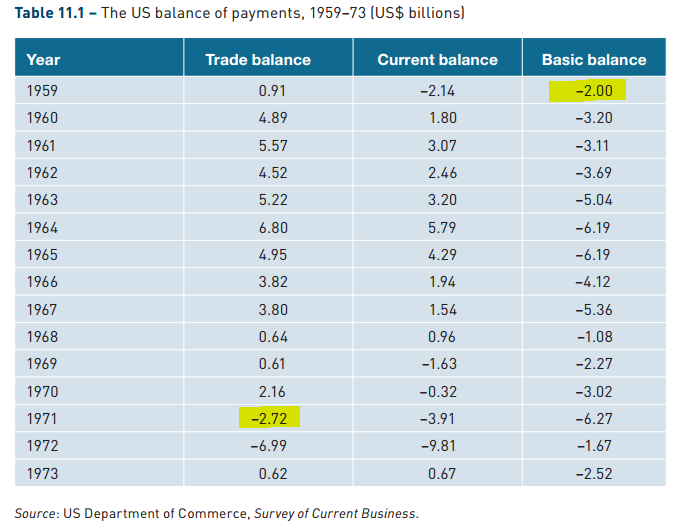
\includegraphics[scale=0.55]{fig/systems/usbop}
\end{frame}
\begin{frame}{Goals and Structure of the IMF}
	\begin{itemize}
		\item a mixture of discipline and flexibility原则性+灵活性
		\item Discipline
			\begin{itemize}
				\item exchange
				rates be fixed to the dollar, which, in turn, was tied to gold
				\item floating exchange rates were a cause of speculative
				instability and were harmful to international trade.
				
			\end{itemize}
		\item Flexibility
			\begin{itemize}
				\item Loans were made from a fund paid for by members in gold
				and currencies.
				\item Each country had a quota, which determined its
				contribution to the fund and the maximum amount it could
				borrow.
				\item Large loans were made conditional on the supervision of
				domestic policies by the IMF: IMF conditionality.
				\item Devaluations could occur if the IMF determined that the				economy was experiencing a “fundamental
				disequilibrium.”
			\end{itemize}
	\end{itemize}
\end{frame}

\begin{frame}{Convertibility and the Expansion of Private Financial Flows}
	\begin{itemize}
		\item \structure{convertible currency} is one that may be freely exchanged for foreign		currencies.
		\item The U.S. and Canadian dollars became convertible in 1945
		\item Because dollars were freely convertible, it became an
		international money.
		\item central banks had
		to be attentive to foreign financial conditions or take the risk that sudden reserve losses
		might leave them without the resources needed to peg exchange rates.
	\end{itemize}
\end{frame}

\begin{frame}{Speculative Capital Flows and Crises}
\begin{itemize}
	\item Current account deficits and surpluses took on added significance under the new
	conditions of increasingly mobile private financial flows.
	\begin{itemize}
		\item A country with a large
		and persistent current account deficit——fundamental disequilibrium——Suspicion of an impending devaluation—— balance of
		payments crisis
		\item countries with large current account surpluses——Propensity of avaluation—— selling the home currency in the
		foreign exchange market to keep the currency from appreciating——money supply grow uncontrollably——内部失衡
	\end{itemize}
	\item 	A record British trade balance deficit in early
	1964 led to a period of intermittent speculation against the pound 
	\item France devalued its franc and Germany revalued its mark in 1969 after similar speculative attacks
\end{itemize}
\end{frame}

\begin{frame}{Analyzing Policy Options for Reaching
	Internal and External Balance}
	\begin{itemize}
		\item Maintaining Internal Balance
		$Y^{f} = C + I + G + CA(EP^{*}/P, A) = A + CA(EP^{*}/P, A)$
		\begin{itemize}
			\item An increase in government purchases (or a
			decrease in taxes) increases aggregate demand
			and output above its full employment level.
			\item To restore internal balance in the short run, a
			revaluation (a fall in E) must occur.
		\end{itemize}
	\end{itemize}
\end{frame}

\begin{frame}{Internal Balance (II),
	External Balance (XX),
	and the “Four Zones of
	Economic Discomfort”}

\begin{columns}[onlytextwidth]
	\begin{column}{0.5\textwidth}
		\begin{itemize}			
		\item The diagram shows what	different levels of the exchange
		rate, $E$, and overall domestic	spending, $A$, imply for
		employment and the current
		account. 
		\item Along II, output is at its
		full-employment level,Y f. 
		\item Along	XX, the current account is at its
		target level, X
		\end{itemize}
	\end{column}
	\begin{column}{0.5\textwidth}
		\centering
		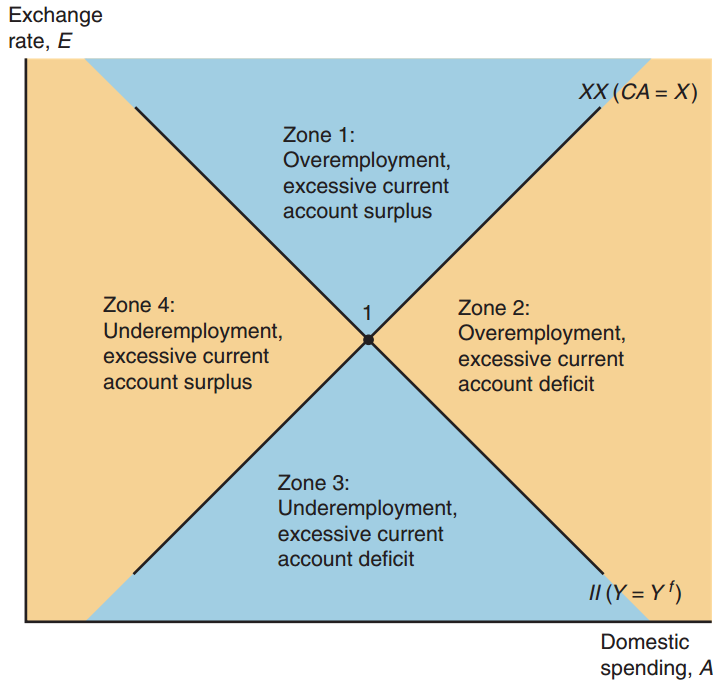
\includegraphics[scale=0.45]{fig/systems/balance}
	\end{column}
\end{columns}
\end{frame}

\begin{frame}{Policies to Bring about Internal and External Balance}

\begin{columns}[onlytextwidth]
	\begin{column}{0.5\textwidth}
		\begin{itemize}			
			\item Suppose the economy is on point 2. What does it represent?
				
			\item How to push it to point 1?
			 
			\item Unless the currency is devalued and			the level of domestic spending rises,			internal and external balance (point 1)			cannot be reached
			\item Acting alone,
			a change in fiscal policy, for example,
			enables the economy to attain either
			internal balance (point 3) or external
			balance (point 4), but only at the cost
			of increasing the economy’s distance
			from the goal that is sacrificed.
		\end{itemize}
	\end{column}
	\begin{column}{0.5\textwidth}
		\centering
		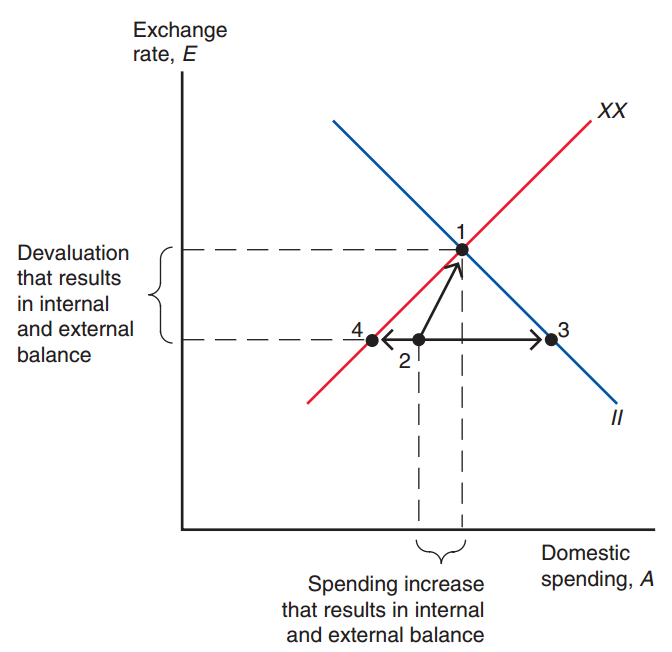
\includegraphics[scale=0.45]{fig/systems/balance2}
	\end{column}
\end{columns}
\end{frame}

\begin{frame}{Why did Bretton Woods system breake down?}
\begin{columns}[onlytextwidth]
	\begin{column}{0.5\textwidth}
		\begin{itemize}			
		\item Confidance Problem——Triffin Problem
		\item Bad money drive out good money——Gresham's Law
		\item Lack of an adjustment mechanism
		\item The seigniorage problem
		\end{itemize}
	\begin{block}{}
		Key point: Other country has to keep Dollar reserve
	\end{block}
	\end{column}
	\begin{column}{0.5\textwidth}
		\centering
		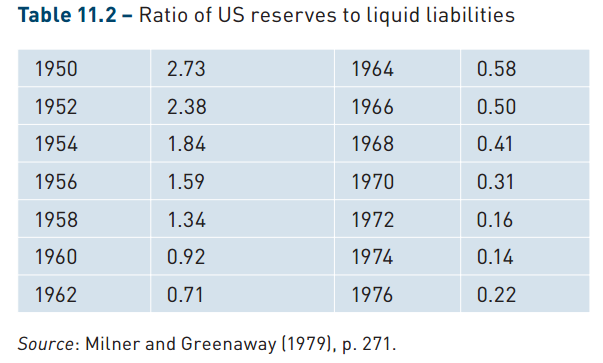
\includegraphics[scale=0.5]{fig/systems/triffin}
	\end{column}
\end{columns}
	
\end{frame}



\section{Post-Bretton Woods Era}
\begin{frame}{1976年牙买加会议}
	\begin{itemize}
		\item 中心议题:提高特别提款权在国际储备中的重要性
		\item 《国际货币基金组织协定第二修正案》于1978年4月正式生效
		\item 赋予各国货币当局在选择汇率制度上的自由裁定权,向IMF汇报其汇率制度即可
		\item 唯一禁止的就是将成员方货币与黄金挂钩
		\item 正式确认了布雷顿森林体系的瓦解
	\end{itemize}
\end{frame}

\begin{frame}{THE SNAKE AND THE EMS蛇形浮动汇率体系和欧洲货币体系}

			\begin{itemize}			
				\item mid-1972-1973, UK, Swiss, Japan decided to let the pound/franc/yen float
				\item 19 March ,1972 the European currencies began a joint float against the	dollar known as the \structure{‘Snake in the Tunnel’}
				\item In June 1973 the Snake in the Tunnel became the \structure{plain Snake}
				\item The snake was replaced by the EMS which commenced operations in 1979(Details in next chapter)
			\end{itemize}
		\centering
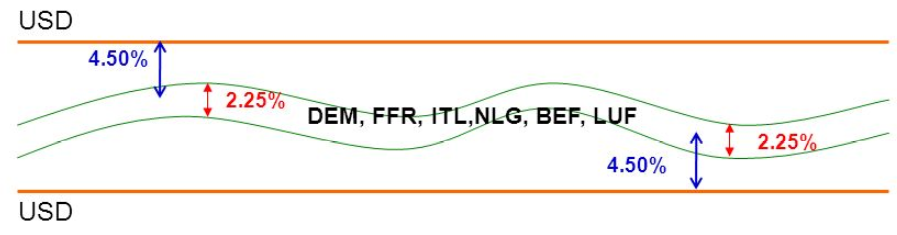
\includegraphics[scale=0.5]{fig/systems/snake}
\end{frame}

\begin{frame}{the Dazzling Dollar, 1980-1985}
\begin{itemize}			
	\item Towards the end of 1978 the Iranian revolution, the second oil shock start, which led
	to a further hike in OPEC oil prices from \$13 a barrel in mid-1978 to \$32 a barrel
	in mid-1980
	\item tight monetary policy + rather relaxed fiscal policy $\longrightarrow$ dollar appreciation $\longrightarrow$  deteriorating balance of payments $\longrightarrow$ protectionist measures threats $\longrightarrow$  the Plaza Accord
		\centering
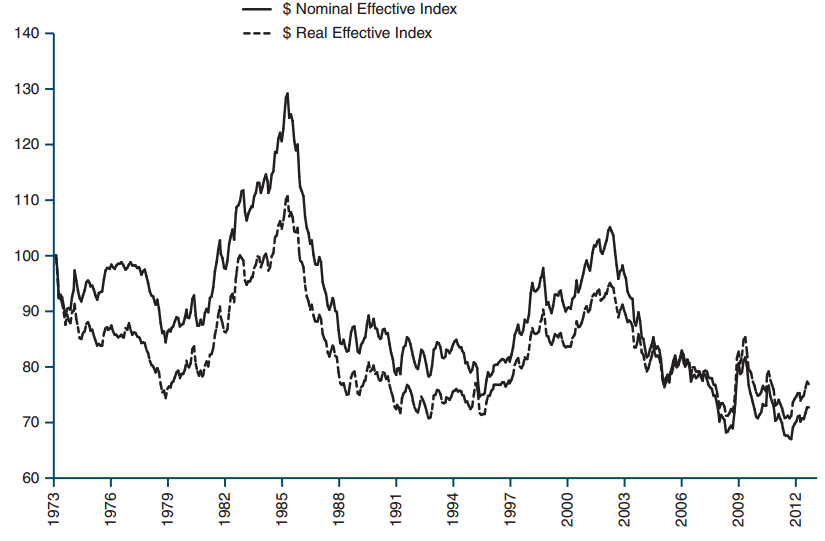
\includegraphics[scale=0.45]{fig/systems/dollar}
\end{itemize}
\end{frame}

\begin{frame}{from Plaza to Louvre and beyond}
	\begin{itemize}
		\item In September 1985, finance ministers and central bank governors from the so-called
		G5 countries (France, West Germany, the United States, the United Kingdom and Japan) met at the Plaza Hotel, New York, and issued a communiqué known as the \structure{Plaza Accord}
		\item  there was a commitment to ‘cooperate more closely to encourage this, when to do so would be helpful’.
		\item  Following the Accord the dollar depreciated throughout 1986
		\item At a G7 meeting held at Paris in February 1987, the finance ministers issued what		is known as the \structure{Louvre Accord}.
		\item  it is believed was aimed at
		keeping the dollar within a 5\% target band against the Deutschmark and the yen.
	\end{itemize}
\end{frame}

\begin{frame}{currency turmoil and crises post-1990}

	\begin{itemize}
		\item The significant loosening of monetary policy following the stockmarket collapse of
		1987 eventually led to renewed pressure on world inflation, which in turn required a
		series of interest rate rises to bring it under control. 
		\item Te early 1990s also witnessed
		unprecedented currency turmoil
		\item The Mexican ‘tequila crisis’ of 1994–95
		\item The 1997–98 Asian crisis
		\item The 1998 Russian crisis
		\item The 1999 Brazilian crisis
		\item The Long-Term Capital Management crisis
		\item The Turkish crisis of 2001
		\item The Argentinian default of 2002
		\item The Eurozone crisis
	\end{itemize}
\end{frame}

\begin{frame}[allowframebreaks]{Reform of the international financial system}
Totally speaking, Te present international monetary system has been called a ‘non-system’ 
	\begin{itemize}
		\item the williamson target zone proposal
		\begin{itemize}
			\item the exchange rate between the major international currencies should be managed within a target zone system
			\item the currency’s ‘fundamental equilibrium effective exchange rate’ (FEEER).基本均衡有效汇率
			\item  A country’s exchange rate would then be allowed to fluctuate within
			a system of \textcolor{red}{‘soft-edged bands’} of ±10\% either side of the FEEER.
			\item they argue that the target zone proposal can	help rule out the possibility of self-fulfilling and destabilizing foreign exchange speculation
		\end{itemize}
		\item the Mckinnon global monetary target proposal
				\begin{itemize}
			\item Ronald McKinnon (1982, 1984) has argued that much exchange rate volatility is
			due to the process of currency substitution. 
			\item  the Friedman rule for smooth monetary growth should be shifted
			from a national to a carefully defi ned international level 各国货币当局强烈干预汇市,平抑市场的过剩需求和供给
			\item There are numerous problems with the McKinnon proposal. For example, fixing the nominal exchange rate at some PPP level
		\end{itemize}
		\item the tobin foreign exchange tax proposal
				\begin{itemize}
			\item James Tobin (1978) has argued that much of the disruptive exchange rate movements
			witnessed under floating regimes have been caused by destabilizing short-term capital flows. 
		\item Tobin suggests that a tax be imposed on all foreign exchange transactions ‘to throw some sand in the wheels of our excessively efficient international		money markets’ . 
		\item  criticisms
		\begin{itemize}
			\item not all short-term capital movements are undesirable, and the tax would prevent
			some stabilizing movements.
			\item with today’s
			modern financial markets it is likely that the tax would be easily circumvented as
			financial innovation would lead to a replication of speculative positions through
			synthetic instruments that were unaffected by the tax.
			\item Government tend to abuse this national monetary autonomy
			\item to avoid the tax there could a greater use of barter trade which is
			notoriously inefficient.
		\end{itemize}
		\end{itemize}
	\end{itemize}
\end{frame}


\begin{frame}{Reform of the international financial architecture}

The aim of the debate on reform of the international financial architecture has been
about reducing the frequency of crises and also the costs, both financial and economic,
when they do occur. 
\begin{itemize}
	\item Is there fundamental flaws in the current international financial system 根本性的缺陷
	\item  the role of the IMF in the international monetary system.  the IMF itself introduces moral hazard. 废除IMF
	\item  the free movement of international capital. 给发展中国家资本账户管制权
	\item Mishkin (1994) and Fischer (1999) argue that there needs	to be a new international agency with credit
	lines ready to make emergency loans to countries being subjected to ‘unwarranted’
	speculative attacks. 国际最后贷款人
	\item an international bankruptcy	court along the lines proposed by Sachs (1995) where nation states with excessive
	debt levels could go to seek some sort of protection from their creditors 国际破产法庭
	
\end{itemize}
\end{frame}

\end{document}


